\section{Evaluation Methodology}
\label{sec:expsetup}



%nd questionnaires were used to discuss their sleep posture during their daily. The main content of the questionnaire was about their common arm position in 4 different sleeping postures.

%\textcolor{blue}{To ensure \systemname supports a representative set of arm positions and sleep postures, we carried out a survey with $100$ randomly chosen volunteers. The results of the survey, together with findings from previous studies~\cite{position2014,HandPosition2}, were used to determine the positions used as the basis for our study of sleep position detection.}% And we also found that the positions of these arms are effective during the training and testing of the algorithm.}



\begin{figure}[!t]
	\centering
	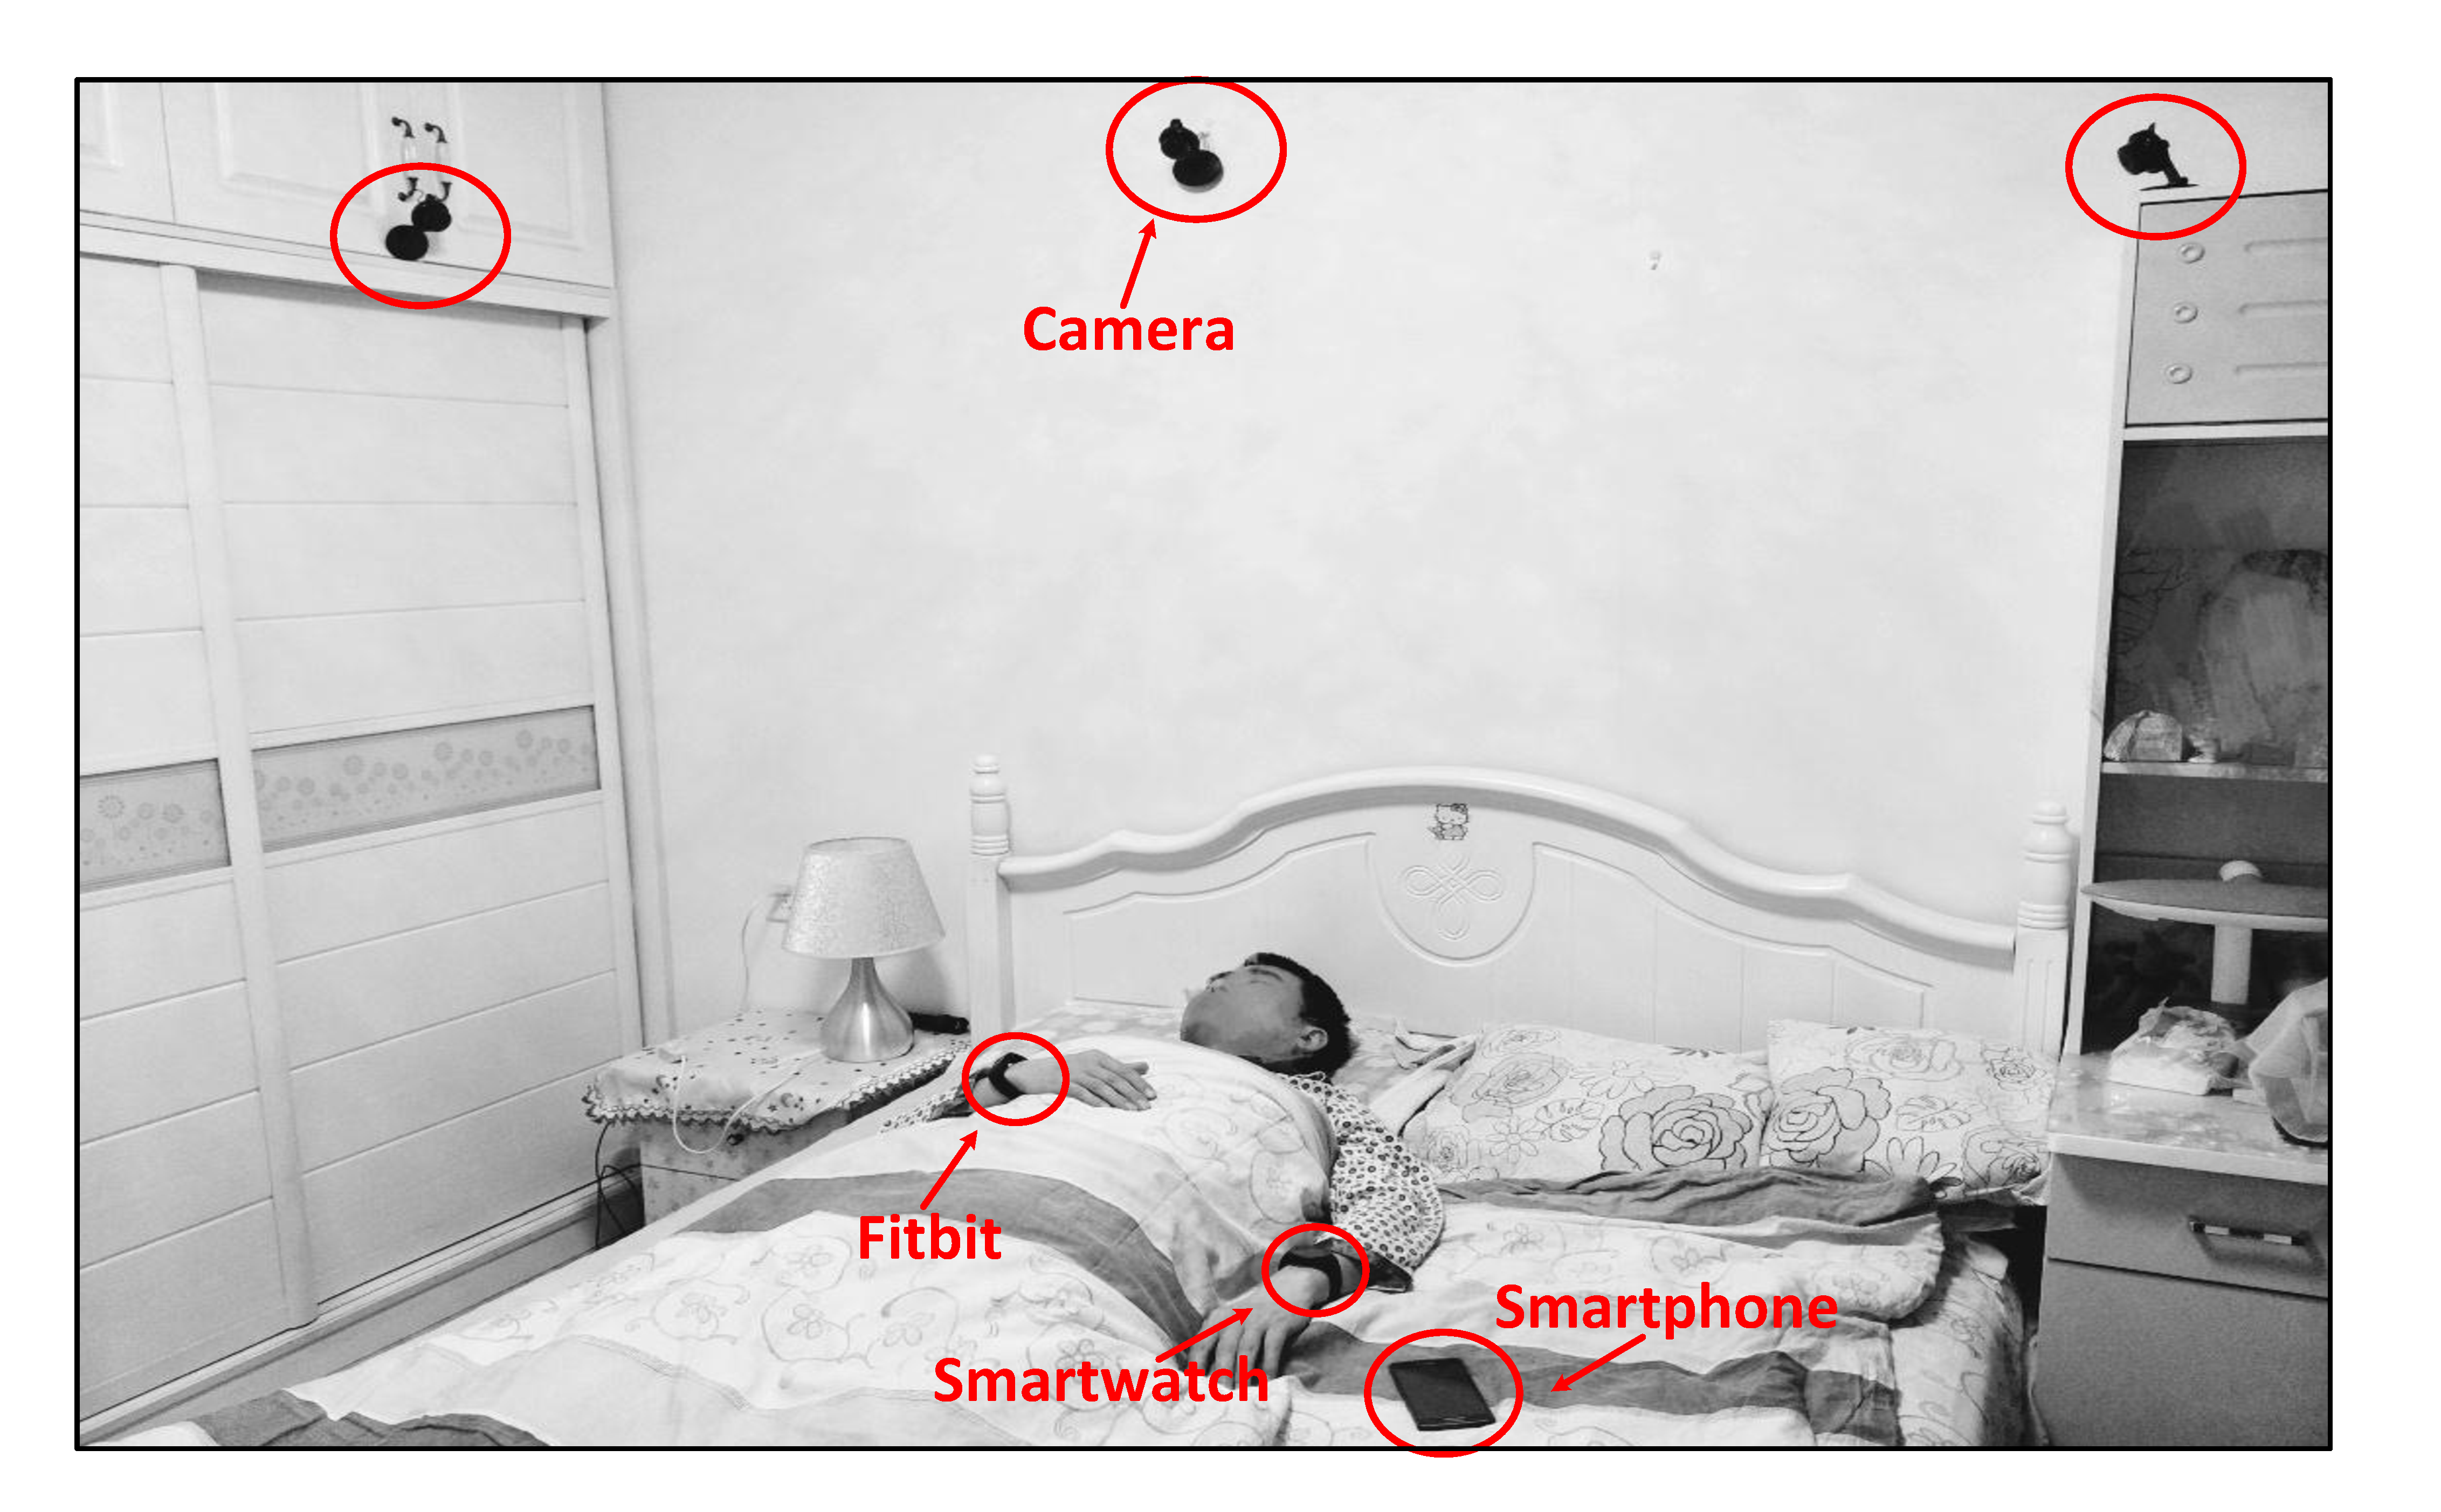
\includegraphics[width=0.75\linewidth]{Figures/setup.pdf}
	\caption{Experimental setup in one of our participants' home. }\label{fig:setup}
\end{figure}



%\section{Experimental Setup} {\systemname} is implemented on the HuaWei Smartwatch 2. The programming platform is JAVA. For simplification,
%we implement the event detection on a laptop and the collected data is processed by MATLAB. \textcolor{blue}{In our experiments, we recruit
%15 volunteers (6 males and 9 females) from 15 years old to 60 years old,  of whom 5 people are between the ages of 15 and 25, and 5 are
%between the ages of 25 and 40, and 6 people between 40 and 60 years old. According to our preliminary survey of participants, two of 40 to
%60 year old are found to have long-term sleep disorders,  one with difficulty falling asleep and having a light sleep with more dreams, and
%another participant with the symptoms of awaking at night and early awakening, and there is a 53-year-old participant have been troubled by
%snoring, they are the focus of our attention. In addition, other participants occasionally suffer some sleep problems such as insomnia,
%snore and so on.} The experiments are conducted over two weeks, and during experiments, these volunteers sleep alone in a quiet room and
%each of them sleeps at least 6 hours. Moreover, each participant is asked to wear a smartwatch and Fitbit Charge2 \cite{fitbit} on his/her
%wrist simultaneously during sleep. And the smartphone with Sleep As Android \cite{SleepAndroid} is placed beside the participant's body.
%Considering that there is no absolute ground truth to detect sleep stage and the operations of other professional medical equipment are
%complicated, we leverage the result of Fitbit Charge2, a comfortable and effortless bracelet, as the ground truth. Sleep As Android, a
%widely used app for sleep detection, run the whole sleep process for comparing with our system. At the same time, to test the reliability
%of our methods, we use the video camera to monitor the sleep, and those recorded data by camera are set as groundtruth during the
%experiment. \textcolor{red}{Fig.00000} illustrates the experimental scene for our system.



\subsection{Experimental Setup\label{sec:evalusers}}

We evaluate \systemname through experiments conducted in $15$ single-occupancy homes over a two-week period.  The participants include 6 males and 9 females, whose age spans 15 to 60 years. To ensure too little sleep had no effect on the results, each participant was required to sleep at least $6$ hours per night during the study period. Two of our participants have been diagnosed with long-term, on-going sleep-related disorders, and one participant has described that his sleep is significantly affected by snoring. The remaining participants reported their sleep quality to go up and down and having poor sleep from time to time. The study was approved by local IRB, and participants were separately asked to consent to release their data for analysis. In total we collected 210 sets of nocturnal sleep data from our participants. %During the experiment, our volunteers slept alone in a bedroom at
%home, and they slept for at least 6 hours per night.

During the study, participants are asked to wear a smartwatch on their wrist. To obtain ground truth of sleep events, three video cameras were placed on the ceiling to monitor the user's sleep activities, as shown in Fig.~\ref{fig:setup}. The cameras have night vision and thus can capture sleep activity with high-quality. The video footage was manually labelled with different sleep activities and the labels were used as ground truth in our evaluation. To demonstrate the overall benefits of \systemname and the events captured by it, we separately collected ground truth information about sleep quality using questionnaires which were administrated each morning. The questionnaires were based on the Pittsburgh Sleep Quality Index (PSQI), a widely used and validated questionnaire in sleep quality research~\cite{buysse1989pittsburgh}. Finally, we collected sleep stage estimates from a Fitbit Charge2 and considered them as ground truth for sleep stage estimation. While the performance of Fitbit is not comparable to medical grade PSG, it has been shown to have a good association in adults~\cite{evenson2015systematic,fitbit01,fitbit02,fitbit03}, especially in estimating REM and light sleep stage. Equipping the participants with PSG was not feasible as it would disrupt their normal sleeping routines and potentially bias and reduce sleep activities, which are the main focus of our work. Moreover, the goal of our experiments is not to demonstrate that \systemname is capable of medical grade sleep monitoring, but to demonstrate that it performs comparably to commercial systems in common sleep monitoring tasks, while at the same time being able to capture much richer set of sleep information.  We also compare our approach against Sleep Hunter~\cite{gu2016sleep}, a state-of-the-art mobile-based sleep monitoring approach, and a
smartphone-based sleep monitoring app named Sleep as Android~\cite{SleepAndroid}. To provide a fair comparison against these baselines, we also place a smartphone next to the user's body on the bed to collect the data for Sleep Hunter and Sleep as Android.
	
%	Instrumenting the users with PSG sensors was not feasible for For sleep stage estimation, we use the stages reported by Fitbit Charge2 which is proven to have . As we know, Fitbit is a commercial state-of-the-art and a popular sleep monitoring wristband. It has less interference with the subject's normal sleep process, making easier for subjects to relax and maintain normal sleep. However, even if PSG has high accuracy in monitoring sleep, it may have some impact on their psychological and normal sleep processes (as it requires the user to wear many instruments) , so as not to reflect the actual sleep conditions. Moreover, Fitbit is inexpensive and easy to deploy, so it is very convenient to apply to our large number of home-style experimental scenarios.} Therefore, our participants are asked to wear two smartwatches on their wrists: a Fitbit Charge2 that runs the Fitbit app and a Huawei Smartwatch 2 that runs \systemname.
\subsection{Pilot Study: Training Data\label{sec:trainingdata}}
\textcolor{cyan}{ To train the models used in our system and to determine optimal parameter values, a small-scale pilot study with $10$ participants was carried out prior to the main experiment.  The training examples used to train our algorithms and to determine the algorithm parameters are collected from 10 users
	(5 males and 5 females). Our testing users were asked to wear a smartwatch to sleep and collected the sensor data
	while they were sleeping. Every testing user contributes 10 nocturnal sleep data over a two-week period. These users were 
	different from those took part in our evaluation} (Section~\ref{sec:evalusers}).



\subsection{Prototype Implementation \label{sec:implementation}}
We prototype and evaluate \systemname on a Huawei Smartwatch 2 wearable device. The smartwatch is equipped with a Quad-core Cortex-A7
processor at 1.1 GHz.  It runs the Android Wear 2.0 operating system. We use five sensors of the smartwatch: the accelerometer, gyroscope,
microphone, light sensor and orientation sensor. To reduce energy consumption of the smartwatch, in the experiments we analyse the sensor data on a a XiaoMI Note2 Android smartphone to which the smartwach sends sensor measurements over Bluetooth. The sensors on the smartwatch are sampled every $30$ms, which was chosen to balance between information quality and energy consumption. \systemname starts tracking sleep events when it detects that the light is off and there has been no body movement for 30 minutes. As part of an initialization process, \systemname estimates the initial body posture and hand position. It then uses these as a starting point to monitor sleep events like the body posture, rollovers, hand positions and body movements.
